\documentclass{article}
\usepackage[utf8]{inputenc}
\usepackage[pdftex]{graphicx}	

\newcommand{\horrule}[1]{\rule{\linewidth}{#1}} 	% Horizontal rule
\title{
	%\vspace{-1in} 	
	\usefont{OT1}{bch}{b}{n}
	\horrule{0.5pt} \\[0.4cm]
	\huge CS150A Homework 2 -- Writing \\
	\horrule{2pt} \\[0.5cm]
}
\author{
	\normalfont 								\normalsize
	School of Information Science and Technology \\
	[-3pt]		\normalsize
	\today
}



\begin{document}
\maketitle

\section{B+ tree Refinement (10 pts)}

How many I/Os would it cost to insert an entry into our table if we had a height 3, unclustered alternative 3 B+ tree in the worst case? Assume that the cache is empty at the beginning and there are at most 6 entries with the same key. And what is the answer for a height 5, clustered alternative 3 B+ tree in the best case? Assume each page is at most 2/3 full. \\   


\section{Relational Algebra (40 pts)}

    As shown in the following figures, there are three instances corresponding to three relations:
Sailors, Reserves and Boats.
\begin{center}
    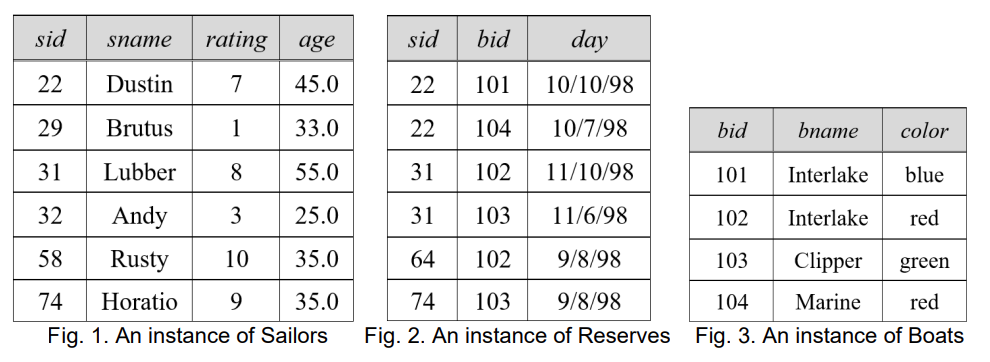
\includegraphics[height =5cm]{RA.png}
\end{center}
Use relational algebra to describe the following queries.
\begin{itemize}
    \item [1.] Find the names of sailors who reserved boats after 10/7/98.\\
    \item [2.] Find the age of sailors who have reserved boat Interlake with blue color. \\
    \item [3.] Find the name of boats which have been reserved by sailors rating 7 or higher.\\
    \item [4.] Find the color of boats which once reserved by sailors Dustin on 10/10/98.\\
    \item [5.] Find the name of sailors who didn't reserved any boat named Marine.\\
\end{itemize}


\section{Joins (10 pts)}
Determine whether each of the following statements is True or False.
\begin{itemize}
    \item [a.] Block Nested Loops join will always perform at least as well as Page Nested Loops Join when it comes to minimizing I/Os.
    \item [b.] Grace hash join is usually the best algorithm for joins in which the join condition includes an inequality.
\end{itemize}

\section{Query Optimization (40 pts)}
Consider two relations R(a, b) and S(a), with 1000 tuples and 500 tuples respectively. We have
an index on R.a with 50 unique integer values uniformly distributed in the range [1, 50], and an index on
S.a with 25 unique integer values uniformly distributed in the range [1, 25]. We do not have an
index on R.b.\\
Use selectivity estimation to estimate the number of tuples produced by the following queries.
\begin{enumerate}
    \item SELECT * FROM R \\ \\
    \item SELECT * FROM R WHERE a = 99 \\ \\
    \item SELECT * FROM R WHERE b = 99 \\ \\
    \item SELECT * FROM R WHERE a $\leq$ 24 \\ \\
    \item SELECT * FROM R WHERE b $\leq$ 10 \\ \\
    \item SELECT * FROM R WHERE NOT a $\leq$ 24 \\ \\
    \item SELECT * FROM R WHERE a $\leq$ 24 AND b $\leq$ 10 \\ \\
    \item SELECT * FROM R WHERE a $\leq$ 24 OR b $\leq$ 10 \\ \\
    \item SELECT * FROM R WHERE a = b \\ \\
    \item SELECT * FROM R, S WHERE R.a = S.a \\ \\
\end{enumerate}

\end{document}
